\documentclass{standalone}
\usepackage{tikz}
\usetikzlibrary{patterns, positioning}


\begin{document}
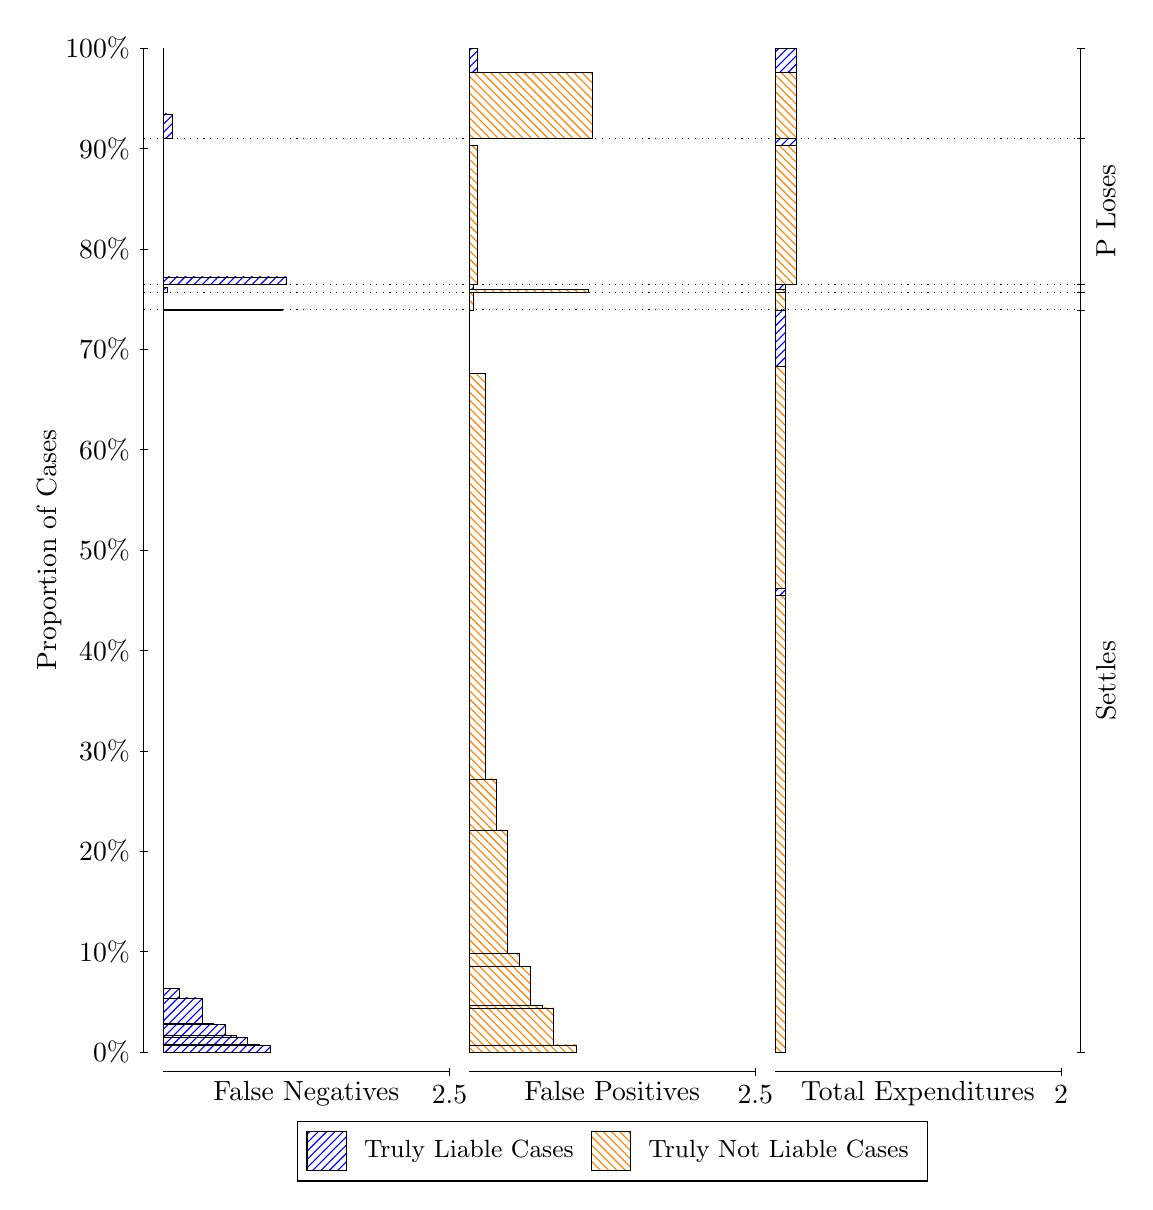
\begin{tikzpicture}
\draw[black, very thin] (1.5,1.75) -- (1.5,14.5);
\node[rotate=90, text=black, anchor=center] at (0.3, 8.125) {Proportion of Cases};
\draw[black, very thin] (1.45,1.75) -- (1.55,1.75);
\node[text=black, anchor=east] at (1.45, 1.75) {0\%};
\draw[black, very thin] (1.45,3.025) -- (1.55,3.025);
\node[text=black, anchor=east] at (1.45, 3.025) {10\%};
\draw[black, very thin] (1.45,4.3) -- (1.55,4.3);
\node[text=black, anchor=east] at (1.45, 4.3) {20\%};
\draw[black, very thin] (1.45,5.575) -- (1.55,5.575);
\node[text=black, anchor=east] at (1.45, 5.575) {30\%};
\draw[black, very thin] (1.45,6.85) -- (1.55,6.85);
\node[text=black, anchor=east] at (1.45, 6.85) {40\%};
\draw[black, very thin] (1.45,8.125) -- (1.55,8.125);
\node[text=black, anchor=east] at (1.45, 8.125) {50\%};
\draw[black, very thin] (1.45,9.4) -- (1.55,9.4);
\node[text=black, anchor=east] at (1.45, 9.4) {60\%};
\draw[black, very thin] (1.45,10.675) -- (1.55,10.675);
\node[text=black, anchor=east] at (1.45, 10.675) {70\%};
\draw[black, very thin] (1.45,11.95) -- (1.55,11.95);
\node[text=black, anchor=east] at (1.45, 11.95) {80\%};
\draw[black, very thin] (1.45,13.225) -- (1.55,13.225);
\node[text=black, anchor=east] at (1.45, 13.225) {90\%};
\draw[black, very thin] (1.45,14.5) -- (1.55,14.5);
\node[text=black, anchor=east] at (1.45, 14.5) {100\%};

\draw[black, very thin] (13.4,1.75) -- (13.4,14.5);
\draw[black, very thin] (13.35,1.75) -- (13.45,1.75);
\node[anchor=west] at (13.35, 1.75) {};
\draw[black, very thin] (13.35,11.175) -- (13.45,11.175);
\node[anchor=west] at (13.35, 11.175) {};
\draw[black, very thin] (13.35,11.396) -- (13.45,11.396);
\node[anchor=west] at (13.35, 11.396) {};
\draw[black, very thin] (13.35,11.502) -- (13.45,11.502);
\node[anchor=west] at (13.35, 11.502) {};
\draw[black, very thin] (13.35,13.354) -- (13.45,13.354);
\node[anchor=west] at (13.35, 13.354) {};
\draw[black, very thin] (13.35,14.5) -- (13.45,14.5);
\node[anchor=west] at (13.35, 14.5) {};

\draw[black, very thin, pattern color=blue, pattern=north east lines] (1.75,1.75) rectangle (3.1125,1.831);
\draw[black, very thin, pattern color=blue, pattern=north east lines] (1.75,1.831) rectangle (2.9672,1.8416);
\draw[black, very thin, pattern color=blue, pattern=north east lines] (1.75,1.8416) rectangle (2.8218,1.9391);
\draw[black, very thin, pattern color=blue, pattern=north east lines] (1.75,1.9391) rectangle (2.6765,1.9563);
\draw[black, very thin, pattern color=blue, pattern=north east lines] (1.75,1.9563) rectangle (2.5312,2.1016);
\draw[black, very thin, pattern color=blue, pattern=north east lines] (1.75,2.1016) rectangle (2.3858,2.1136);
\draw[black, very thin, pattern color=blue, pattern=north east lines] (1.75,2.1136) rectangle (2.2405,2.4382);
\draw[black, very thin, pattern color=blue, pattern=north east lines] (1.75,2.4382) rectangle (1.9498,2.5551);
\draw[black, very thin, pattern color=orange, pattern=north west lines] (1.75,2.5551) rectangle (1.75,11.175);
\draw[black, very thin, pattern color=blue, pattern=north east lines] (1.75,11.175) rectangle (3.2578,11.177);
\draw[black, very thin, pattern color=orange, pattern=north west lines] (1.75,11.177) rectangle (1.75,11.396);
\draw[black, very thin, pattern color=blue, pattern=north east lines] (1.75,11.396) rectangle (1.8045,11.462);
\draw[black, very thin, pattern color=orange, pattern=north west lines] (1.75,11.462) rectangle (1.75,11.502);
\draw[black, very thin, pattern color=blue, pattern=north east lines] (1.75,11.502) rectangle (3.3123,11.594);
\draw[black, very thin, pattern color=orange, pattern=north west lines] (1.75,11.594) rectangle (1.75,13.354);
\draw[black, very thin, pattern color=blue, pattern=north east lines] (1.75,13.354) rectangle (1.859,13.663);
\draw[black, very thin, pattern color=orange, pattern=north west lines] (1.75,13.663) rectangle (1.75,14.5);
\draw[black, very thin, pattern color=orange, pattern=north west lines] (5.6333,1.75) rectangle (6.9958,1.8399);
\draw[black, very thin, pattern color=orange, pattern=north west lines] (5.6333,1.8399) rectangle (6.7052,2.3113);
\draw[black, very thin, pattern color=orange, pattern=north west lines] (5.6333,2.3113) rectangle (6.5598,2.3387);
\draw[black, very thin, pattern color=orange, pattern=north west lines] (5.6333,2.3387) rectangle (6.4145,2.8363);
\draw[black, very thin, pattern color=orange, pattern=north west lines] (5.6333,2.8363) rectangle (6.2692,3.0017);
\draw[black, very thin, pattern color=orange, pattern=north west lines] (5.6333,3.0017) rectangle (6.1238,4.5711);
\draw[black, very thin, pattern color=orange, pattern=north west lines] (5.6333,4.5711) rectangle (5.9785,5.2195);
\draw[black, very thin, pattern color=orange, pattern=north west lines] (5.6333,5.2195) rectangle (5.8332,10.37);
\draw[black, very thin, pattern color=blue, pattern=north east lines] (5.6333,10.37) rectangle (5.6333,11.175);
\draw[black, very thin, pattern color=orange, pattern=north west lines] (5.6333,11.175) rectangle (5.6878,11.393);
\draw[black, very thin, pattern color=blue, pattern=north east lines] (5.6333,11.393) rectangle (5.6333,11.396);
\draw[black, very thin, pattern color=orange, pattern=north west lines] (5.6333,11.396) rectangle (7.1412,11.436);
\draw[black, very thin, pattern color=blue, pattern=north east lines] (5.6333,11.436) rectangle (5.6878,11.502);
\draw[black, very thin, pattern color=orange, pattern=north west lines] (5.6333,11.502) rectangle (5.7423,13.262);
\draw[black, very thin, pattern color=blue, pattern=north east lines] (5.6333,13.262) rectangle (5.6333,13.354);
\draw[black, very thin, pattern color=orange, pattern=north west lines] (5.6333,13.354) rectangle (7.1957,14.191);
\draw[black, very thin, pattern color=blue, pattern=north east lines] (5.6333,14.191) rectangle (5.7423,14.5);
\draw[black, very thin, pattern color=orange, pattern=north west lines] (9.5167,1.75) rectangle (9.6529,7.5484);
\draw[black, very thin, pattern color=blue, pattern=north east lines] (9.5167,7.5484) rectangle (9.6529,7.64);
\draw[black, very thin, pattern color=orange, pattern=north west lines] (9.5167,7.64) rectangle (9.6529,10.461);
\draw[black, very thin, pattern color=blue, pattern=north east lines] (9.5167,10.461) rectangle (9.6529,11.175);
\draw[black, very thin, pattern color=orange, pattern=north west lines] (9.5167,11.175) rectangle (9.6529,11.393);
\draw[black, very thin, pattern color=blue, pattern=north east lines] (9.5167,11.393) rectangle (9.6529,11.396);
\draw[black, very thin, pattern color=orange, pattern=north west lines] (9.5167,11.396) rectangle (9.6529,11.436);
\draw[black, very thin, pattern color=blue, pattern=north east lines] (9.5167,11.436) rectangle (9.6529,11.502);
\draw[black, very thin, pattern color=orange, pattern=north west lines] (9.5167,11.502) rectangle (9.7892,13.262);
\draw[black, very thin, pattern color=blue, pattern=north east lines] (9.5167,13.262) rectangle (9.7892,13.354);
\draw[black, very thin, pattern color=orange, pattern=north west lines] (9.5167,13.354) rectangle (9.7892,14.191);
\draw[black, very thin, pattern color=blue, pattern=north east lines] (9.5167,14.191) rectangle (9.7892,14.5);
\draw[black, dotted] (1.5,11.175) -- (13.4,11.175);
\draw[black, dotted] (1.5,11.396) -- (13.4,11.396);
\draw[black, dotted] (1.5,11.502) -- (13.4,11.502);
\draw[black, dotted] (1.5,13.354) -- (13.4,13.354);
\draw[black, very thin] (1.75,1.5) -- (5.3833,1.5);
\node[text=black, anchor=north] at (3.5667, 1.5) {False Negatives};
\draw[black, very thin] (5.3833,1.45) -- (5.3833,1.55);
\node[text=black, anchor=north] at (5.3833, 1.45) {2.5};

\draw[black, very thin] (5.6333,1.5) -- (9.2667,1.5);
\node[text=black, anchor=north] at (7.45, 1.5) {False Positives};
\draw[black, very thin] (9.2667,1.45) -- (9.2667,1.55);
\node[text=black, anchor=north] at (9.2667, 1.45) {2.5};

\draw[black, very thin] (9.5167,1.5) -- (13.15,1.5);
\node[text=black, anchor=north] at (11.333, 1.5) {Total Expenditures};
\draw[black, very thin] (13.15,1.45) -- (13.15,1.55);
\node[text=black, anchor=north] at (13.15, 1.45) {2};

\node[text=black, centered, rotate=90] at (13.72, 6.4623) {Settles};


\node[text=black, centered, rotate=90] at (13.72, 12.428) {P Loses};


\draw (7.449999999999999,1.5) node[draw=none] (baseCoordinate) {};
\begin{scope}[align=center]
        \matrix[scale=0.5, draw=black, below=0.5cm of baseCoordinate, nodes={draw}, column sep=0.1cm]{
            \node[rectangle, draw, minimum width=0.5cm, minimum height=0.5cm, pattern color=blue, pattern=north east lines] {}; &
            \node[draw=none, font=\small, text=black] (B) {Truly Liable Cases}; &
            \node[rectangle, draw, minimum width=0.5cm, minimum height=0.5cm, pattern color=orange, pattern=north west lines] {}; &
            \node[draw=none, font=\small, text=black] (B) {Truly Not Liable Cases}; \\
            };
\end{scope}

\end{tikzpicture}
\end{document}